\documentclass[a4paper,10pt]{article}
\usepackage[utf8]{inputenc}
\usepackage{tikz}
\usetikzlibrary{arrows,decorations.pathmorphing,backgrounds,positioning,fit,petri}
\renewcommand*{\familydefault}{\sfdefault}

\tikzset{forestyle/.style = {rectangle, fill = black!20, thick, minimum width = 5cm, minimum height = 0.5cm, text width = 4.5cm, outer sep = 1mm}, 
	backstyle/.style = {rectangle, fill = black, minimum width = 5cm, minimum height = 0.5cm}, 
	pre/.style={<-, shorten <=1pt, >=stealth, ultra thick}}


\begin{document}

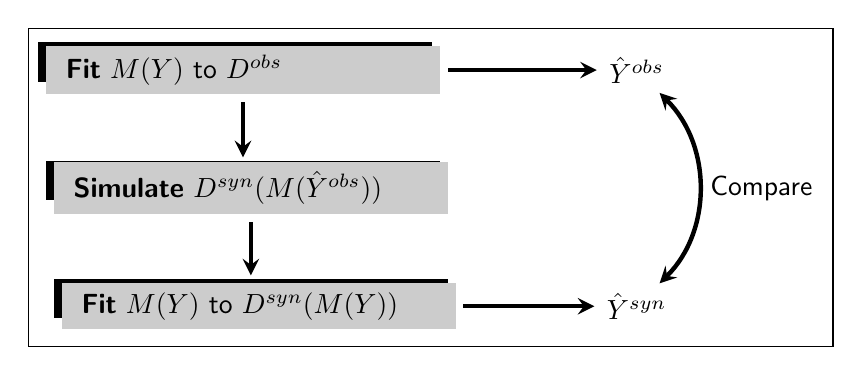
\begin{tikzpicture}

 \node (fade1) at (-0.1, 0.1) [backstyle] {};
 \node (step1) at (0,0) [forestyle] {\textbf{Fit} $M(Y)$ to $D^{obs}$};
 \node (estimated) at (5,0)  {$\hat{Y}^{obs}$}
  edge [pre] (step1);
 
 \node (fade2) at (0, -1.4) [backstyle] {}
  edge [pre] (step1);
 \node (step2) at (0.1, -1.5) [forestyle] {\textbf{Simulate} $D^{syn}(M(\hat{Y}^{obs}))$};
 
 \node (fade3) at (0.1, -2.9) [backstyle] {}
  edge [pre] (step2);
 \node (step3) at (0.2, -3) [forestyle] {\textbf{Fit} $M(Y)$ to $D^{syn}(M(Y))$};
 \node (synthetic) at (5,-3) {$\hat{Y}^{syn}$}
  edge [pre] (step3)
  edge [<->, ultra thick, bend right = 45, >=stealth] node[auto,swap] (compare) {Compare} (estimated);

 \begin{scope}[on background layer]
  \node [draw = black, semithick,
  fit = (fade1) (step1) (estimated) (fade2) (step2) (fade3) (step3) (synthetic) (compare)] {};
 \end{scope}

 
\end{tikzpicture}

\end{document}
